\documentclass[10pt,a4paper]{amsart}
\usepackage[margin=19mm]{geometry}
\usepackage{amsmath,amssymb,mathtools}
\usepackage[scr=rsfs,cal=euler]{mathalfa}
\usepackage{xfrac}
\usepackage[unicode,hidelinks,bookmarks=false]{hyperref}
\newcommand{\ie}{i.e.\ }
\newcommand{\cf}{cf.\ }
\newcommand{\resp}{respectively\ }
\newcommand{\Subsection}{\subsection}
\providecommand{\nobreakdash}{\nobreak\hbox{-}}
\setlength{\emergencystretch}{2em}
\multlinegap0pt
\usepackage{mathrsfs}
\usepackage{indentfirst}
\usepackage{setspace}
\usepackage{tikz}
\usepackage{float}
\usepackage{colortbl}
\usepackage{multirow}
\setlength{\oddsidemargin}{0.35in}
\setlength{\evensidemargin}{0.35in}
\setlength{\topmargin}{-0.5cm}
\definecolor{sectionlink}{RGB}{0,100,200}
\newtheorem{theo}{Theorem}[section]
\newtheorem{lem}{Lemma}[section]
\newtheorem{prop}{Proposition}[section]
\newtheorem{cor}{Corollary}[section]
\newtheorem{rem}{Remark}[section]
\newcommand{\vmid}{\mid}
\newcommand{\ol}{\overline}
\newcommand{\ul}{\underline}
\numberwithin{equation}{section}
\begin{document}
\title[Sharp Coefficient Estimates for the Exponential Starlike cla]{Sharp Coefficient Estimates for the Exponential Starlike class $\mathcal{S}_{ex}^{\ast}$}
\author{Pradip Das; Nabadwip Sarkar}
\date{}
\maketitle
\noindent\emph{Source and licence.} Sharp Coefficient Estimates for the Exponential Starlike class $\mathcal{S}_{ex}^{\ast}$. Version arXiv:2606.10186v4 (CC BY 4.0). This material is distributed under the Creative Commons Attribution 4.0 International licence, http://creativecommons.org/licenses/by/4.0/, as recorded in the arXiv OAI licence metadata for this exact version and shown on the abstract page https://arxiv.org/abs/2606.10186v4. Full rights notice: licenses/arxiv-2606.10186-CC-BY-4.0.txt.\par\smallskip
\noindent\textit{Editorial scope.} Counted unit: the original \texttt{theo} environment \texttt{T1} at source lines 542--579 together with its complete proof at lines 581--1209; the delivered document keeps source lines 130--1649 so that every referenced label and every citation resolves inside it. Native editable source is the paper's own concatenated TeX; the AMS wrapper is editorial formatting only. No publisher class, upstream script or unrelated artwork is redistributed.
\begin{equation}\label{eq1}
f(z)=z+\sum_{n=2}^{\infty}a_n z^n,\qquad z\in\mathbb{D}.
\end{equation}
that is, if it satisfies $f(0)=0$ and $f'(0)=1$. Let $\mathcal{S}\subset\mathcal{A}$ denote the usual subclass of univalent functions. We say that $f\in\mathcal{A}$ is starlike if its image $f(\mathbb{D})$ is starlike with respect to the origin. The class $\mathcal{S}^*$ of starlike functions is characterized analytically by
\[
f\in\mathcal{S}^*
\iff
\Re\left(\frac{zf'(z)}{f(z)}\right)>0,\qquad z\in\mathbb{D}.
\]
For the basic theory of univalent functions, we refer to the monographs of Duren \cite{PLD1} and Goodman \cite{G}.

Let $\Omega$ denote the class of Schwarz functions $\omega$ analytic in $\mathbb{D}$ with $\omega(0)=0$ and $|\omega(z)|<1$ for $z\in\mathbb{D}$. A function $f$ is subordinate to another analytic function $g$, written $f\prec g$, if there exists $\omega\in\Omega$ such that
\[
f(z)=g(\omega(z)),\qquad z\in\mathbb{D}.
\]
When $g$ is univalent, this is equivalent to the geometric condition
\[
f(0)=g(0),\qquad f(\mathbb{D})\subset g(\mathbb{D}).
\]
The notion of subordination is classical and plays a central role in geometric function theory; see, for example, Pommerenke \cite{Pommerenke1971}.

Ma and Minda \cite{MM} used subordination to give a unified treatment of many starlike and convex classes. They introduced the class
\[
\mathcal{S}^{*}(\phi)
:=
\left\{
f\in\mathcal{S}:
\frac{zf'(z)}{f(z)}\prec \phi(z),\ z\in\mathbb{D}
\right\},
\]
where $\phi$ is analytic and univalent in $\mathbb{D}$, $\Re\phi(z)>0$, $\phi(0)=1$, $\phi'(0)>0$, and $\phi(\mathbb{D})$ is symmetric about the real axis.

Coefficient problems for univalent functions have a long history, beginning with the Bieberbach conjecture, which was ultimately proved by de Branges \cite{LDB1}. Earlier contributions include Goluzin's distortion theorems \cite{G1}, Hayman's work on successive coefficients \cite{H}, and Grinspan's estimates for adjacent coefficients \cite{G2}. Among the many coefficient functionals studied in the literature, logarithmic coefficients have received considerable attention because of their close links with the geometry of univalent mappings and with the Schwarzian derivative. For $f\in\mathcal{S}$, the logarithmic coefficients $\gamma_n$ are defined by
\[
\log\frac{f(z)}{z}
=
2\sum_{n=1}^{\infty}\gamma_n z^n,\qquad z\in\mathbb{D}.
\]
Recent results on logarithmic coefficients and their differences have been obtained, for instance, by Obradovi\'c and Tuneski \cite{Obradovic2024}, Lecko and Partyka \cite{Lecko2023}, and Kumar and Cho \cite{Kumar2023}. Sharp bounds for successive coefficients and their differences have also been investigated by Leung \cite{Leung1978}, Li and Sugawa \cite{LiSugawa}, Peng and Obradovi\'c \cite{Peng2019}, and Arora and collaborators \cite{Arora2019,Arora2022,Arora2023}.

Recently, subclasses of starlike functions associated with exponential mappings have attracted much interest. The class $\mathcal{S}_e^*$ corresponding to the exponential function $e^z$ was introduced by Mendiratta et al.\ \cite{Mendiratta2015}. Later, Panja et al.\ \cite{Panja2026} studied classes governed by
\[
\phi(z)=e^{\alpha z},\qquad 0<\alpha\le1.
\]
Accordingly, a normalized function $f\in\mathcal{A}$ belongs to the class $\mathcal{S}_{ex}^{\ast}$ if it satisfies
\begin{equation}\label{subordination}
\frac{zf'(z)}{f(z)}\prec e^{\alpha z},\qquad z\in\mathbb{D}.
\end{equation}
Sharp bounds for Hermitian--Toeplitz determinants in the class $\mathcal{S}_e^*$ were obtained by Sarkar \cite{Sarkar}, while inverse logarithmic coefficient bounds were recently established by Das and Sarkar \cite{DasSarkar2026}. Higher-order Schwarzian derivative estimates for related classes were studied in \cite{Das2026a,Srivastava2026}.

The function $\phi(z)=e^{\alpha z}$ satisfies all standard Ma--Minda conditions: it is univalent, has positive real part in $\mathbb{D}$, is symmetric with respect to the real axis, and maps $\mathbb{D}$ onto a convex oval-shaped domain. As $\alpha$ increases from $0$ to $1$, the domain $\phi(\mathbb{D})$ expands continuously from a neighborhood of $w=1$ to a larger convex region. This behavior is illustrated in Figure~\ref{fig_domain}.

\begin{figure}[htbp]
\centering
\begin{tikzpicture}[scale=1.8, >=stealth]
    % Left Scope: The Domain D in the z-plane
    \begin{scope}[shift={(-2.2,0)}]
        \draw[->, gray!70, line width=0.6pt] (-1.4,0) -- (1.5,0) node[right, black] {$\Re(z)$};
        \draw[->, gray!70, line width=0.6pt] (0,-1.4) -- (0,1.4) node[above, black] {$\Im(z)$};
        
        \fill[blue!6, opacity=0.5] (0,0) circle (1);
        \draw[thick, blue!70!black] (0,0) circle (1);
        
        \node at (0,0) [below left] {$0$};
        \fill (0,0) circle (1.2pt);
        \fill (1,0) circle (1.2pt) node[below right] {$1$};
        \fill (-1,0) circle (1.2pt) node[below left] {$-1$};
        
        \node at (0.4,0.4) [blue!70!black, font=\bfseries] {$\mathbb{D}$};
        \node at (0,-1.7) [black] {\small $z$-plane};
    \end{scope}

    % Mapping Arrow with enhanced labeling
    \draw[->, thick, black!80] (-0.7,0.2) .. controls (-0.3,0.4) and (0.3,0.4) .. (0.7,0.2) 
        node[midway, above=2pt, black, font=\small] {$\phi(z) = e^{\alpha z}$};

    % Right Scope: Nested Target Domains in the w-plane
    \begin{scope}[shift={(2.2,0)}]
        \draw[->, gray!70, line width=0.6pt] (-0.4,0) -- (3.3,0) node[right, black] {$\Re(w)$};
        \draw[->, gray!70, line width=0.6pt] (0,-1.4) -- (0,1.4) node[above, black] {$\Im(w)$};
        
        % 1. Outer domain: alpha = 1.0 (Deep purple)
        \fill[purple!15, opacity=0.4] plot[domain=0:360, samples=180, variable=\t] 
            ({exp(1.0*cos(\t))*cos(1.0*sin(\t) r)}, {exp(1.0*cos(\t))*sin(1.0*sin(\t) r)});
        \draw[thick, purple!80!black] plot[domain=0:360, samples=180, variable=\t] 
            ({exp(1.0*cos(\t))*cos(1.0*sin(\t) r)}, {exp(1.0*cos(\t))*sin(1.0*sin(\t) r)});

        % 2. Intermediate domain: alpha = 0.75 (Plum)
        \fill[purple!25, opacity=0.4] plot[domain=0:360, samples=180, variable=\t] 
            ({exp(0.75*cos(\t))*cos(0.75*sin(\t) r)}, {exp(0.75*cos(\t))*sin(0.75*sin(\t) r)});
        \draw[thick, dashed, purple!60!black] plot[domain=0:360, samples=180, variable=\t] 
            ({exp(0.75*cos(\t))*cos(0.75*sin(\t) r)}, {exp(0.75*cos(\t))*sin(0.75*sin(\t) r)});

        % 3. Inner domain: alpha = 0.5 (Orchid/Pink)
        \fill[magenta!20, opacity=0.5] plot[domain=0:360, samples=180, variable=\t] 
            ({exp(0.5*cos(\t))*cos(0.5*sin(\t) r)}, {exp(0.5*cos(\t))*sin(0.5*sin(\t) r)});
        \draw[thick, dotted, magenta!80!black] plot[domain=0:360, samples=180, variable=\t] 
            ({exp(0.5*cos(\t))*cos(0.5*sin(\t) r)}, {exp(0.5*cos(\t))*sin(0.5*sin(\t) r)});
            
        % Core baseline points
        \node at (0,0) [below left] {$0$};
        \fill (0,0) circle (1.2pt);
        \fill (1,0) circle (1.2pt) node[below left] {$1$}; 
        
        % Dynamic boundary intercepts for alpha = 1.0
        \fill ({exp(1)},0) circle (1.2pt) node[below right] {$e^{1}$};
        \fill ({exp(-1)},0) circle (1.2pt) node[above left=1pt] {\small $e^{-1}$};
        
        % Legend/Labels directly inside the spaces
        \node at (2.1,0.5) [purple!90!black, font=\scriptsize, fill=white, inner sep=1pt, rounded corners=1pt] {$\alpha=1.0$};
        \node at (1.5,0.75) [purple!70!black, font=\scriptsize] {$\alpha=0.75$};
        \node at (1.1,0.35) [magenta!90!black, font=\scriptsize] {$\alpha=0.5$};
        
        \node at (2.5,1.1) [purple!80!black, font=\bfseries] {$\phi(\mathbb{D})$};
        \node at (1.2,-1.7) [black] {\small $w$-plane};
    \end{scope}
\end{tikzpicture}
\caption{Evolution of the image domain $\phi(\mathbb{D})$ for the parameter values $\alpha \in \{0.5, 0.75, 1.0\}$.}
\label{fig_domain}
\end{figure}

\subsection{Inverse logarithmic coefficients}

Let $f\in\mathcal{S}$. The inverse logarithmic coefficients $\Gamma_n$, introduced by Ponnusamy et al.\ \cite{Ponnusamy2018}, are defined via the expansion of the inverse function $f^{-1}$:
\[
F_{f^{-1}}(w)
:=
\log\frac{f^{-1}(w)}{w}
=
2\sum_{n=1}^{\infty}\Gamma_n w^n
\]
near $w=0$. These coefficients are the natural inverse analogue of the logarithmic coefficients and have been studied extensively because of their connections with the Bieberbach conjecture and the geometry of univalent mappings. Several authors have investigated inverse logarithmic coefficients and related Hankel and Toeplitz determinants; see, for example, \cite{MandalAhamed2024,MandalAhamed2026,MandalAhamedZaprawa2025}.

The first four inverse logarithmic coefficients can be expressed directly in terms of the Taylor coefficients $a_n$ of $f$ as
\begin{equation}\label{IG1}
\begin{cases}
\Gamma_1=-\dfrac{1}{2}a_2,\\[8pt]
\Gamma_2=-\dfrac{1}{2}a_3+\dfrac{3}{4}a_2^2,\\[8pt]
\Gamma_3=-\dfrac{1}{2}\left(a_4-4a_2a_3+\dfrac{10}{3}a_2^3\right),\\[8pt]
\Gamma_4=\dfrac{35}{8}a_2^4-\dfrac{15}{2}a_2^2a_3+\dfrac{5}{2}a_2a_4+\dfrac{5}{4}a_3^2-\dfrac{1}{2}a_5.
\end{cases}
\end{equation}

Ponnusamy et al.\ \cite{Ponnusamy2018} proved that, for the full class $\mathcal{S}$, the inverse logarithmic coefficients satisfy the sharp bound
\[
|\Gamma_n|
\le
\frac{1}{2n}\binom{2n}{n},\qquad n\in\mathbb{N},
\]
with equality for the Koebe function and its rotations. This result motivates the search for sharper bounds within important subclasses of $\mathcal{S}$.

Hankel and Toeplitz determinants involving logarithmic coefficients have also been intensively investigated. These determinants provide useful information about the structure of coefficient sequences and have applications in operator theory, signal processing, and random matrix theory. Kowalczyk and Lecko~\cite{12,15} introduced the logarithmic Hankel determinants
\[
H_{q,n}\left(F_f/2\right)
=
\begin{vmatrix}
\gamma_n & \gamma_{n+1} & \cdots & \gamma_{n+q-1}\\
\gamma_{n+1} & \gamma_{n+2} & \cdots & \gamma_{n+q}\\
\vdots & \vdots & \ddots & \vdots\\
\gamma_{n+q-1} & \gamma_{n+q} & \cdots & \gamma_{n+2(q-1)}
\end{vmatrix}.
\]
The corresponding inverse analogue
\[
H_{q,n}\bigl(F_{f^{-1}}/2\bigr)
=
\begin{vmatrix}
\Gamma_n & \Gamma_{n+1} & \cdots & \Gamma_{n+q-1}\\
\Gamma_{n+1} & \Gamma_{n+2} & \cdots & \Gamma_{n+q}\\
\vdots & \vdots & \ddots & \vdots\\
\Gamma_{n+q-1} & \Gamma_{n+q} & \cdots & \Gamma_{n+2(q-1)}
\end{vmatrix}
\]
was studied in~\cite{10,16}. Hankel determinant bounds for special subclasses have also been obtained by Sim et al.\ \cite{STZ} and Tang et al.\ \cite{TAA,TAH}.

Similarly, Hermitian--Toeplitz determinants, which are Hermitian analogues of classical Toeplitz determinants, have become important in coefficient problems for analytic functions. The theory of Toeplitz matrices goes back to Hartman and Wintner \cite{HW}; see also Kucerovsky et al.\ \cite{KMS}. In the context of univalent functions, Hermitian--Toeplitz determinants have been studied for numerous subclasses, including starlike, convex, bounded turning, and Janowski-type functions; see \cite{Ali,C,K3,KKD2023,KPR,KumarCho2021,KSC,GJSS2023,TKBSKS2025,UFBCL2025}.

Although logarithmic coefficient problems and Hankel determinant bounds have been studied for some exponential subclasses~\cite{Panja2026}, the inverse logarithmic functionals for the full parametric family $\mathcal{S}_{ex}^{\ast}$ remain largely open. In particular, the dependence on the parameter $\alpha$ produces a multi-branch structure that requires a careful case-by-case optimization.

The purpose of this paper is to give a unified treatment of sharp coefficient estimates for the class $\mathcal{S}_{ex}^{\ast}$ governed by $\phi(z)=e^{\alpha z}$, $0<\alpha\le1$. More precisely, we establish the following sharp results.

\begin{enumerate}
\item Sharp upper bounds for the initial inverse logarithmic coefficients $\Gamma_1$, $\Gamma_2$, and $\Gamma_3$. A key feature of our work is the four-branch structure of the bound for $|\Gamma_3|$, with transition values
\[
\alpha_* \approx 0.542712,\qquad
\alpha_b \approx 0.679103,\qquad
\alpha_c \approx 0.691095.
\]

\item Sharp upper and lower bounds for the successive coefficient difference
\[
|\Gamma_2|-|\Gamma_1|.
\]

\item Sharp bounds for the second-order inverse logarithmic Hankel determinant
\[
H_{2,1}\bigl(F_{f^{-1}}/2\bigr)
=
\Gamma_1\Gamma_3-\Gamma_2^2.
\]

\item Sharp upper and lower bounds for the third-order Hermitian--Toeplitz determinant $T_{3,1}(f)$. The lower bound changes at
\[
\alpha_H = \frac{-1+\sqrt{241}}{15} \approx 0.9683,
\]
and it reduces to the known value $-\frac{1}{15}$ when $\alpha=1$, thereby extending previous results for the class $\mathcal{S}_e^*$.

\item A complete solution of the generalized Fekete--Szeg\H{o} problem for
\[
|a_3-\lambda a_2^2|-\mu|a_2|,
\]
following the recent investigations of Lecko and Partyka \cite{Lecko2024} and Bulboac\u{a} et al.\ \cite{Bulboaca2025}.
\end{enumerate}

All estimates are sharp, and the corresponding extremal functions are constructed explicitly. Our approach relies on the Carath\'eodory parametrization of functions with positive real part, the Libera--Z{\l}otkiewicz parametrization \cite{LZ}, and on optimization lemmas due to Cho et al.\ \cite{C12}, Choi et al.\ \cite{CKS1}, Ma and Minda \cite{MM}, and Sim and Thomas \cite{SimThomas2020}. The extremal functions are obtained from the integral representation
\[
f(z)
=
z\exp\left(
\int_0^z \frac{1}{t}
\left[
\exp\left(
\alpha\frac{p(t)-1}{p(t)+1}
\right)
-1
\right]
dt
\right),
\]
where $p\in\mathcal{P}$ is a suitable Carath\'eodory function.

The paper is organized as follows. In Section~2, we recall the auxiliary lemmas needed in the proofs. Section~3 contains sharp bounds for the inverse logarithmic coefficients $\Gamma_1$, $\Gamma_2$, and $\Gamma_3$. In Section~4, we prove sharp bounds for the difference $|\Gamma_2|-|\Gamma_1|$. Section~5 is devoted to the second-order inverse logarithmic Hankel determinant. In Section~6, we obtain sharp upper and lower bounds for the third-order Hermitian--Toeplitz determinant. Section~7 contains the complete solution of the generalized Fekete--Szeg\H{o} problem. Finally, Section~8 summarizes the main results and outlines possible future directions.
\section{Auxiliary lemmas}

Let $\mathcal{P}$ denote the class of all analytic functions $p$ in the unit disk $\mathbb{D}$ satisfying $p(0) = 1$ and $\Re p(z) > 0$ for all $z \in \mathbb{D}$. Every $p \in \mathcal{P}$ admits the series representation
\begin{equation}\label{p1}
p(z) = 1 + \sum_{n=1}^{\infty} p_n z^n, \quad z \in \mathbb{D}.
\end{equation}
Functions in $\mathcal{P}$ are referred to as \emph{Carath\'{e}odory functions}. It is well-known that for $p \in \mathcal{P}$, the coefficients satisfy the sharp bound $|p_n| \le 2$ for all $n \ge 1$ (see \cite{PLD1}).

Now we recall the following well-known lemma due to Cho et al. \cite{C12}.
\begin{lem}\label{L1} \cite[Lemma 2.4]{C12} If $p\in\mathcal{P}$ is of the form (\ref{p1}), then
\begin{equation}\label{c1}p_1 =2\tau_1,\end{equation}
\begin{equation}\label{c2} p_2=2\tau_1^2 + 2(1 - |\tau_1|^2)\tau_2\end{equation}
and
\begin{equation}\label{c3} p_3 = 2\tau_1^3+4(1-|\tau_1|^2)\tau_1\tau_2 - 2(1 - |\tau_1|^2)\ol{\tau_1}\tau_2^2 + 2(1 - \tau_1^2)(1 - |\tau_2|^2)\tau_3
\end{equation}
for some $\tau_1, \tau_2, \tau_3 \in\mathbb{\ol D}:= \{z \in \mathbb{C}: |z| \le 1 \}$.
For $ \tau_1 \in \mathbb{T} := \{ z \in \mathbb{C} : |z| = 1 \} $, there is a unique function $ p \in \mathcal{P} $ with $ p_1 $ as in (\ref{c1}), namely,
\[
p(z) = \frac{1 + \tau_1 z}{1 - \tau_1 z}, \quad z \in \mathbb{D}.
\]
For $ \tau_1 \in \mathbb{D} $ and $ \tau_2 \in \mathbb{T} $, there is a unique function $ p \in \mathcal{P} $ with $ p_1 $ and $ p_2 $ as in (\ref{c1}) and (\ref{c2}), namely,
\[
p(z) = \frac{1 + (\ol \tau_1 \tau_2 + \tau_1) z + \tau_2 z^2}{1 + (\ol \tau_1 \tau_2 - \tau_1) z - \tau_2 z^2}, \quad z \in \mathbb{D}.
\]
For $ \tau_1, \tau_2 \in \mathbb{D} $ and $ \tau_3 \in \mathbb{T} $, there is a unique function $ p \in \mathcal{P} $ with $ p_1 $, $ p_2 $, and $ p_3 $ as in (\ref{c1}-\ref{c3}), namely,
\[
p(z) = \frac{1 + (\ol\tau_2 \tau_3 + \ol\tau_1 \tau_2 + \tau_1)z+(\ol\tau_1\tau_3+\tau_1\ol\tau_2\tau_3+\tau_2)z^2+\tau_3z^3}{1+(\ol\tau_2\tau_3+\ol\tau_1\tau_2-\tau_1)z+(\ol\tau_1\tau_3-\tau_1\ol\tau_2\tau_3-\tau_2)z^2-\tau_3z^3},\;\;z\in\mathbb{D}
\]
\end{lem}

Following a well-known result due to Choi et al. \cite{CKS1}.
\begin{lem}\label{L2}\cite{CKS1} Let $A$, $B$, $C$ be real numbers and let
\[Y(A, B, C):= \max\limits_{z\in \ol{\mathbb{D}}}\left\lbrace |A+Bz+Cz^2|+1-|z|^2\right\rbrace.\]
\begin{enumerate} 
\item[(i)] If $AC\ge 0$, then
\[Y(A, B, C) =
\begin{cases}
|A|+|B|+|C|, & \text{if}\;\;\; |B|\ge 2(1-|C|), \\
1+|A|+\frac{B^2}{4(1-|C|)}, &\text{if}\;\;\; |B|<2(1-|C|).
\end{cases}
\]
\item[(ii)] If $AC<0$, then 
\[Y(A,B,C)=
\begin{cases}
1-|A|+\frac{B^2}{4(1-|C|)}, &\text{if}\;\;\; -4AC(C^{-2}-1) \le B^2\; \text{and}\; |B|<2(1-|C|), \\
1+|A|+\frac{B^2}{4(1+|C|)}, &\text{if}\;\;\; B^2<\min\left\{4(1+|C|)^2, -4AC(C^{-2}-1) \right\}, \\
R(A,B,C), &\text{otherwise},
\end{cases}
\]
where
\[R(A,B,C):=
\begin{cases}
|A|+|B|-|C|, & \text{if}\;\;\; |C|(|B|+4|A|) \le |AB|, \\
-|A|+|B|+|C|, & \text{if}\;\;\; |AB|\le |C|(|B|-4|A|), \\
(|C|+|A| )\sqrt{1-\frac{B^2}{4AC}}, &\text{otherwise}.
\end{cases}
\]
\end{enumerate} 
\end{lem}

\begin{lem}\label{L3} \cite{MM}
Let $p \in \mathcal{P}$ be given by \eqref{p1}. Then
\[
\left| p_2 - v p_1^2 \right| \le 
\begin{cases}
-4v + 2, & v < 0, \\
2, & 0 \le v \le 1, \\
4v - 2, & v > 1.
\end{cases}
\]
Moreover, for $v < 0$ or $v > 1$, equality holds if and only if
\[
h(z) = \frac{1+z}{1-z} \quad \text{or one of its rotations}.
\]
For $0 < v < 1$, equality holds if and only if
\[
h(z) = \frac{1+z^2}{1-z^2} \quad \text{or one of its rotations}.
\]
\end{lem}

\begin{lem}\label{L6}\cite{SimThomas2020}
Let $J, K,$ and $L$ be numbers such that $J \ge 0$, $K \in \mathbb{C}$, and $L \in \mathbb{R}$. 
Let $p \in \mathcal{P}$ be of the form (\ref{p1}) and define a function by
\[
\Phi(p_1,p_2) = \big| K p_1^2 + L p_2 \big| - \big| J p_1 \big|.
\]
Then 
\[
\Phi(p_{1}, p_{2}) \le 
\begin{cases}
|4K + 2L| - 2J, & \text{if } |2K + L| \ge |L| + J, \\[6pt]
2|L|, & \text{otherwise.}
\end{cases}
\]
and
\[
- \Phi(p_1,p_2) \le 
\begin{cases}
2J - M, & \text{when } J \ge M + 2|L|, \\[6pt]
2J \sqrt{\dfrac{ 2|L|}{M + 2|L|}}, & \text{when } J^2 \le 2|L|(M + 2|L|), \\[10pt]
2|L| +\dfrac{ J^2}{M + 2|L|}, & \text{otherwise}
\end{cases}
\]
where $M=|4K+2L|$.
\end{lem}

We need the following elementary sign lemma to prove Theorem \eqref{T3}:

\begin{lem}\label{lem:Hsign}
For $0<\alpha\le 1$, let $\widetilde H$ be defined by \eqref{Htilde}, and set
\[
d=\alpha^2,\qquad d_0:=\frac{2688}{3395}.
\]
Then $\widetilde H$ has no zero in $(0,1)$ at which it changes sign from positive to negative. More precisely:
\begin{itemize}
\item[(i)] if $0<d\le d_0$, then $\widetilde H(y)<0$ for all $y\in[0,1)$;
\item[(ii)] if $d_0<d\le1$, then $\widetilde H$ is strictly increasing on $[0,1]$, with
\[
\widetilde H(0)<0<\widetilde H(1),
\]
and $\widetilde H$ has a unique zero in $(0,1)$, across which its sign changes from negative to positive.
\end{itemize}
\end{lem}

\begin{proof}[Proof of Lemma]
Write
\[
\widetilde H(y)=A y^3+B y^2+C y-7344,
\]
where
\[
A=384-1120d,\qquad B=528-420d,\qquad C=15120d-4320.
\]
Also
\[
\widetilde H(0)=-7344<0,
\qquad
\widetilde H(1)=13580d-10752
=4(3395d-2688).
\]

We split the proof into two cases.

\paragraph{Case 1: $0<d\le \frac{12}{35}$.}
Then $A\ge0$ and
\[
\widetilde H(1)\le 4\left(3395\cdot \frac{12}{35}-2688\right)
=4(1164-2688)<0.
\]

If $0<d\le \frac27$, then $C\le0$ and $B>0$. Hence $\widetilde H'$ has one negative and one positive root, so $\widetilde H$ first decreases and then increases. Since $\widetilde H(0)<0$ and $\widetilde H(1)<0$, it follows that $\widetilde H(y)<0$ for all $y\in[0,1]$.

If $\frac27<d\le \frac{12}{35}$, then $A>0$, $B>0$, and $C>0$. Thus $\widetilde H'(y)>0$ for all $y\ge0$. Hence $\widetilde H$ is strictly increasing on $[0,1]$, and since $\widetilde H(1)<0$, we again have $\widetilde H(y)<0$ for all $y\in[0,1]$.

\paragraph{Case 2: $\frac{12}{35}<d\le1$.}
Then
\[
A<0,\qquad B>0,\qquad C>0.
\]
Moreover,
\[
\widetilde H'(0)=C=15120d-4320>0,
\]
and
\[
\widetilde H'(1)=3A+2B+C=10920d-2112>0.
\]
Since $\widetilde H'$ is a concave down quadratic and is positive at both endpoints $0$ and $1$, it is positive on the whole interval $[0,1]$. Therefore $\widetilde H$ is strictly increasing on $[0,1]$.

If $\frac{12}{35}<d\le d_0$, then $\widetilde H(1)\le0$, so $\widetilde H(y)<0$ for all $y\in[0,1)$.

If $d_0<d\le1$, then $\widetilde H(0)<0<\widetilde H(1)$. Hence $\widetilde H$ has a unique zero in $(0,1)$, and its sign changes from negative to positive.

Thus in all cases $\widetilde H$ never changes sign from positive to negative on $(0,1)$.
\end{proof}



\section{Sharp Bounds for the Inverse Logarithmic Coefficients}


\begin{theo}\label{T1}
Let $0<\alpha\le 1$. If $f\in \mathcal{S}_{ex}^{\ast}$, then the inverse logarithmic coefficients $\Gamma_n$ $(n=1,2,3)$ satisfy the following sharp inequalities:
\[
|\Gamma_1|\le \frac{\alpha}{2},
\]
\[
|\Gamma_2|\le
\begin{cases}
\dfrac{\alpha}{4}, & 0<\alpha\le \dfrac23,\\[6pt]
\dfrac{3\alpha^2}{8}, & \dfrac23<\alpha\le1,
\end{cases}
\]
and
\begin{equation}\label{ND3}
|\Gamma_3|\le 
\begin{cases}
\dfrac{\alpha}{6}, & 0<\alpha\le \alpha_\star,\\[8pt]
\dfrac{\alpha(7\alpha+2)}{18}
\sqrt{\dfrac{2(7\alpha+2)}{29\alpha^2+42\alpha+12}},
& \alpha_\star<\alpha\le \alpha_b,\\[8pt]
\dfrac{29\alpha(49\alpha^2-16)^{3/2}}
{2232\sqrt{29\alpha^2-12}},
& \alpha_b<\alpha<\alpha_c,\\[8pt]
\dfrac{29\alpha^3}{72}, & \alpha_c\le \alpha\le 1,
\end{cases}
\end{equation}
where
\[
\begin{aligned}
\alpha_\star &\approx 0.542712
\quad \text{is the unique positive root of } 686\alpha^3+327\alpha^2-210\alpha-92=0,\\[2mm]
\alpha_b &\approx 0.679103
\quad \text{is the unique positive root of } 1421\alpha^3+812\alpha^2-712\alpha-336=0,\\[2mm]
\alpha_c &=\sqrt{\frac{928}{1943}}\approx 0.691095.
\end{aligned}
\]
All bounds are sharp for every $\alpha\in(0,1]$.
\end{theo}

\begin{proof}
For $f\in\mathcal{S}_{ex}^{\ast}$, write
\[
\frac{zf'(z)}{f(z)}=e^{\alpha\omega(z)},
\]
where $\omega\in\Omega$. Taking
\[
\omega(z)=\frac{p(z)-1}{p(z)+1},
\qquad
p(z)=1+\sum_{n=1}^{\infty} p_n z^n\in\mathcal{P},
\]
and comparing coefficients gives
\begin{align}
a_2&=\frac{\alpha p_1}{2},\label{ND7}\\
a_3&=\frac{\alpha p_2}{4}
+\frac{3\alpha^2-2\alpha}{16}p_1^2,\label{ND8}\\
a_4&=\frac{\alpha p_3}{6}
+\frac{5\alpha^2-4\alpha}{24}p_1p_2
+\frac{17\alpha^3-30\alpha^2+12\alpha}{288}p_1^3.\label{ND9}
\end{align}

The inverse logarithmic coefficients satisfy
\[
\Gamma_1=-\frac12 a_2,\qquad
\Gamma_2=-\frac12 a_3+\frac34 a_2^2,\qquad
\Gamma_3=-\frac12\left(a_4-4a_2a_3+\frac{10}{3}a_2^3\right).
\]
Hence
\[
|\Gamma_1|=\frac{\alpha}{4}|p_1|\le \frac{\alpha}{2},
\]
and
\[
\Gamma_2
=-\frac{\alpha}{8}p_2
+\frac{3\alpha^2+2\alpha}{32}p_1^2.
\]
Thus
\[
|\Gamma_2|
=\frac{\alpha}{8}
\left|p_2-\frac{3\alpha+2}{4}p_1^2\right|.
\]
Applying Lemma~\ref{L3}, we obtain
\[
|\Gamma_2|\le \frac{\alpha}{4}
\]
for $0<\alpha\le \frac23$, and
\[
|\Gamma_2|\le \frac{3\alpha^2}{8}
\]
for $\frac23<\alpha\le 1$.

We now estimate $|\Gamma_3|$. Substituting \eqref{ND7}--\eqref{ND9} into the expression for $\Gamma_3$ gives
\begin{equation}\label{ND11}
\Gamma_3
=
-\frac{\alpha}{12}p_3
+\frac{7\alpha^2+4\alpha}{48}p_1p_2
-\frac{29\alpha^3+42\alpha^2+12\alpha}{576}p_1^3.
\end{equation}

By rotational invariance of $\mathcal{P}$, we may assume $p_1\in[0,2]$. Put
\[
p_1=2\tau_1,\qquad \tau_1\in[0,1].
\]
Using Lemma~\ref{L1}, write
\[
p_2=2\tau_1^2+2(1-\tau_1^2)\tau_2,
\]
and
\[
p_3
=
2\tau_1^3
+4(1-\tau_1^2)\tau_1\tau_2
-2(1-\tau_1^2)\tau_1\tau_2^2
+2(1-\tau_1^2)(1-|\tau_2|^2)\tau_3,
\]
where $\tau_2,\tau_3\in\overline{\mathbb{D}}$.

Then
\begin{equation}\label{ND12}
\begin{aligned}
|\Gamma_3|
=
\frac{\alpha}{12}\Bigg|
&-\frac{29\alpha^2}{6}\tau_1^3
+7\alpha(1-\tau_1^2)\tau_1\tau_2\\
&+2(1-\tau_1^2)\tau_1\tau_2^2
-2(1-\tau_1^2)(1-|\tau_2|^2)\tau_3
\Bigg|.
\end{aligned}
\end{equation}

If $\tau_1=1$, then $p_1=p_2=p_3=2$, and
\[
|\Gamma_3|=\frac{29\alpha^3}{72}.
\]
If $\tau_1=0$, then
\[
|\Gamma_3|=\frac{\alpha}{12}|-2\tau_3|
\le \frac{\alpha}{6}.
\]

Assume $0<\tau_1<1$. Applying the triangle inequality to \eqref{ND12} gives
\begin{equation}\label{ND13}
|\Gamma_3|
\le
\frac{\alpha(1-\tau_1^2)}{6}
\left(
|A+B\tau_2+C\tau_2^2|+1-|\tau_2|^2
\right),
\end{equation}
where
\[
A=\frac{29\alpha^2\tau_1^3}{12(1-\tau_1^2)}>0,
\qquad
B=-\frac{7\alpha}{2}\tau_1,
\qquad
C=-\tau_1.
\]
Since $AC<0$, we apply Lemma~\ref{L2}(ii).

Define
\[
t_1=\frac{4}{7\alpha+4},
\qquad
t_d=\sqrt{\frac{84}{203\alpha^2+232\alpha+84}}.
\]

\paragraph{Subcase (a).}
The conditions are
\[
|B|<2(1-|C|),\qquad -4AC(C^{-2}-1)\le B^2.
\]
The first inequality is equivalent to $\tau_1<t_1$, while the second is always true because
\[
\frac{29}{3}<\frac{49}{4}.
\]
Thus Subcase (a) applies for $0<\tau_1<t_1$. In this case,
\[
Y_a(\tau_1)
=
1-A+\frac{B^2}{4(1-|C|)}.
\]
Hence
\[
F_a(\tau_1)
:=
\frac{\alpha(1-\tau_1^2)}{6}Y_a(\tau_1)
=
\frac{\alpha}{6}
+
\left(\frac{49\alpha^3}{96}-\frac{\alpha}{6}\right)\tau_1^2
+
\frac{31\alpha^3}{288}\tau_1^3.
\]
Differentiating,
\[
F_a'(\tau_1)
=
\frac{\alpha\tau_1}{96}
\left(
31\alpha^2\tau_1+98\alpha^2-32
\right).
\]
Thus $F_a$ has no interior maximum on $(0,t_1)$. Therefore
\[
\sup_{0<\tau_1<t_1} F_a(\tau_1)
=
\max\left\{
\frac{\alpha}{6},
F_0(\alpha)
\right\},
\]
where
\[
F_0(\alpha)
=
\frac{\alpha^2(1029\alpha^2+1238\alpha+336)}
{9(7\alpha+4)^3}.
\]

\paragraph{Subcase (b).}
The required condition
\[
B^2<-4AC(C^{-2}-1)
\]
becomes
\[
\frac{49}{4}<\frac{29}{3},
\]
which is impossible. Hence Subcase (b) is inactive.

\paragraph{Subcase (c).}
The conditions are
\[
|B|\ge 2(1-|C|),\qquad |C|(|B|+4|A|)\le |AB|.
\]
The first gives $\tau_1\ge t_1$. The second becomes
\[
(203\alpha^2-232\alpha+84)\tau_1^2\ge 84.
\]
For $0<\alpha\le1$,
\[
203\alpha^2-232\alpha+84<84,
\]
so this inequality is impossible. Hence Subcase (c) is inactive.

\paragraph{Subcase (d).}
The conditions are
\[
|B|\ge 2(1-|C|),\qquad |AB|\le |C|(|B|-4|A|).
\]
The first gives $\tau_1\ge t_1$. The second gives $\tau_1\le t_d$. Since $t_1<t_d$ for all $\alpha\in(0,1]$, Subcase (d) applies on $[t_1,t_d]$. In this case,
\[
Y_d(\tau_1)
=
-|A|+|B|+|C|.
\]
Therefore,
\[
F_d(\tau_1)
:=
\frac{\alpha(1-\tau_1^2)}{6}Y_d(\tau_1)
=
-\frac{29\alpha^3}{72}\tau_1^3
+
\frac{\alpha(7\alpha+2)}{12}\tau_1(1-\tau_1^2).
\]
Differentiating,
\[
F_d'(\tau_1)
=
\frac{\alpha}{24}
\left(
2(7\alpha+2)
-(29\alpha^2+42\alpha+12)\tau_1^2
\right).
\]
Hence the critical point is
\[
\tau_d^*
=
\sqrt{
\frac{2(7\alpha+2)}
{29\alpha^2+42\alpha+12}
}.
\]
Since $F_d''(\tau_1)<0$ for $\tau_1>0$, $F_d$ is concave.

Define $\beta$ and $\alpha_b$ by
\[
\tau_d^*(\beta)=t_1(\beta),\qquad
\tau_d^*(\alpha_b)=t_d(\alpha_b).
\]
Equivalently,
\[
343\beta^3+258\beta^2-112\beta-64=0,
\]
so $\beta\approx 0.529607$, and
\[
1421\alpha_b^3+812\alpha_b^2-712\alpha_b-336=0,
\]
so $\alpha_b\approx 0.679103$.
Thus the maximum of $F_d$ on $[t_1,t_d]$ is
\[
F_d^{\max}(\alpha)
=
\begin{cases}
F_0(\alpha), & 0<\alpha\le \beta,\\[6pt]
F_d(\tau_d^*), & \beta<\alpha\le \alpha_b,\\[6pt]
F_d(t_d), & \alpha_b<\alpha\le1.
\end{cases}
\]
A direct computation gives
\[
F_d(\tau_d^*)
=
\frac{\alpha(7\alpha+2)}{18}
\sqrt{
\frac{2(7\alpha+2)}
{29\alpha^2+42\alpha+12}
}.
\]

\paragraph{Subcase (e).}
This subcase applies for $t_d<\tau_1<1$. By Lemma~\ref{L2},
\[
F_e(\tau_1)
=
\frac{\alpha}{72\sqrt{116}}
\left(
12+(29\alpha^2-12)\tau_1^2
\right)
\sqrt{147-31\tau_1^2}.
\]
Set
\[
H(x)=[F_e(\sqrt{x})]^2,\qquad x=\tau_1^2.
\]
Then
\[
H(x)
=
\frac{\alpha^2}{72^2\cdot 116}
\left[
12+(29\alpha^2-12)x
\right]^2
(147-31x).
\]
Differentiating,
\[
H'(x)
=
\frac{\alpha^2}{72^2\cdot116}
\left[
12+(29\alpha^2-12)x
\right]
S(x),
\]
where
\[
S(x)
=
8526\alpha^2-3900-(2697\alpha^2-1116)x.
\]
The first factor is positive for $0\le x\le1$, so the monotonicity of $H$ is controlled by $S(x)$.

The zero of $S$ is
\[
x_e^*
=
\frac{2842\alpha^2-1300}{899\alpha^2-372}.
\]
Also,
\[
S(1)
=
3(1943\alpha^2-928),
\]
so $\alpha_c$ is defined by
\[
\alpha_c^2=\frac{928}{1943}.
\]
A direct calculation gives
\[
S(t_d^2)
=
\frac{
(1218\alpha+696)
(1421\alpha^3+812\alpha^2-712\alpha-336)
}
{203\alpha^2+232\alpha+84}.
\]
Therefore:
\begin{itemize}
\item for $0<\alpha\le\alpha_b$, $S(t_d^2)\le0$ and $S(1)<0$, so $S(x)\le0$ on $[t_d^2,1]$; hence $F_e$ is decreasing and its maximum is at $t_d$;
\item for $\alpha_b<\alpha<\alpha_c$, $S(t_d^2)>0$ and $S(1)<0$, so $x_e^*\in(t_d^2,1)$; hence the maximum of $F_e$ occurs at $x_e^*$;
\item for $\alpha_c\le\alpha\le1$, $S(t_d^2)\ge0$ and $S(1)\ge0$, so $S(x)\ge0$ on $[t_d^2,1]$; hence $F_e$ is increasing and its maximum is at $1$.
\end{itemize}
Thus
\[
\widetilde F_e(\alpha)
:=
\max_{t_d\le \tau_1\le1} F_e(\tau_1)
=
\begin{cases}
F_d(t_d), & 0<\alpha\le\alpha_b,\\[6pt]
F_e(\sqrt{x_e^*}), & \alpha_b<\alpha<\alpha_c,\\[6pt]
F_e(1)=\dfrac{29\alpha^3}{72}, & \alpha_c\le\alpha\le1.
\end{cases}
\]
Moreover,
\[
F_e(\sqrt{x_e^*})
=
\frac{29\alpha(49\alpha^2-16)^{3/2}}
{2232\sqrt{29\alpha^2-12}}.
\]

\subsection*{Phase transition analysis}

The global maximum is
\[
M(\alpha)
=
\max\left\{
\frac{\alpha}{6},
F_0(\alpha),
F_d^{\max}(\alpha),
\widetilde F_e(\alpha),
\frac{29\alpha^3}{72}
\right\}.
\]

\paragraph{Region I: $0<\alpha\le\alpha_\star$.}
Let
\[
R(\alpha)
=
1029\alpha^3+712\alpha^2-336\alpha-192.
\]
Then
\[
\frac{\alpha}{6}-F_0(\alpha)
=
-\frac{\alpha R(\alpha)}{18(7\alpha+4)^3}.
\]
Since $R(0)=-192<0$ and $R(0.55)>0$, the polynomial $R$ has exactly one positive root, $\alpha_0\approx 0.542829$. Since $\beta\approx 0.529607<\alpha_0$,
\[
\frac{\alpha}{6}>F_0(\alpha)
\]
for $0<\alpha\le\beta$.

For $\beta<\alpha\le\alpha_\star$,
\[
F_0(\alpha)=F_d(t_1)\le F_d(\tau_d^*).
\]
Let
\[
Q(\alpha)
=
686\alpha^3+327\alpha^2-210\alpha-92.
\]
Then $\alpha_\star$ is the unique positive root of $Q$. Also,
\[
\left(\frac{\alpha}{6}\right)^2
-
F_d(\tau_d^*)^2
=
-\frac{\alpha^2 Q(\alpha)}
{324(29\alpha^2+42\alpha+12)}.
\]
Since $Q(\alpha)<0$ for $0<\alpha<\alpha_\star$,
\[
\frac{\alpha}{6}\ge F_d(\tau_d^*).
\]
Finally,
\[
\frac{\alpha}{6}
-
\frac{29\alpha^3}{72}
=
\frac{\alpha}{72}(12-29\alpha^2)>0
\]
for $\alpha\le\alpha_\star$. Therefore
\[
M(\alpha)=\frac{\alpha}{6}
\]
for $0<\alpha\le\alpha_\star$.

\paragraph{Region II: $\alpha_\star<\alpha\le\alpha_b$.}
For $\alpha>\alpha_\star$, $Q(\alpha)>0$, so
\[
F_d(\tau_d^*)>\frac{\alpha}{6}.
\]
Also,
\[
F_d(\tau_d^*)^2-F_0(\alpha)^2>0.
\]
Thus $F_d(\tau_d^*)$ dominates $F_0(\alpha)$.

For $\alpha\le\alpha_b$,
\[
\widetilde F_e(\alpha)=F_d(t_d)\le F_d(\tau_d^*).
\]
Finally,
\[
F_d(\tau_d^*)^2
-
\left(\frac{29\alpha^3}{72}\right)^2
>0
\]
for $\alpha\le\alpha_b$. Therefore
\[
M(\alpha)=F_d(\tau_d^*)
\]
for $\alpha_\star<\alpha\le\alpha_b$.

\paragraph{Region III: $\alpha_b<\alpha<\alpha_c$.}
For this range,
\[
F_d(\tau_d^*)>F_0(\alpha),\qquad
F_d(\tau_d^*)>\frac{\alpha}{6}.
\]
A direct calculation gives
\[
\left(
\frac{F_e(\sqrt{x_e^*})}
{F_d(\tau_d^*)}
\right)^2-1
=
\frac{
(1421\alpha^2+434\alpha-340)
(1421\alpha^3+812\alpha^2-712\alpha-336)^2
}
{30752(7\alpha+2)^3(29\alpha^2-12)}
>0.
\]
Thus
\[
F_e(\sqrt{x_e^*})>F_d(\tau_d^*).
\]
Also,
\[
F_e(\sqrt{x_e^*})^2
-
\left(\frac{29\alpha^3}{72}\right)^2
=
\frac{
841\alpha^2(5\alpha^2-1)(67\alpha^2-32)^2
}
{1245456(29\alpha^2-12)}
>0.
\]
Therefore
\[
M(\alpha)=F_e(\sqrt{x_e^*})
\]
for $\alpha_b<\alpha<\alpha_c$.

\paragraph{Region IV: $\alpha_c\le\alpha\le1$.}
For $\alpha\ge\alpha_c$, $S(x)\ge0$ on $[t_d^2,1]$, so
\[
\widetilde F_e(\alpha)=F_e(1)=\frac{29\alpha^3}{72}.
\]
Also,
\[
\frac{29\alpha^3}{72}\ge \frac{\alpha}{6},\qquad
\frac{29\alpha^3}{72}\ge F_0(\alpha),
\]
and
\[
\left(\frac{29\alpha^3}{72}\right)^2
-
F_d(t_d)^2
\ge0.
\]
Hence
\[
M(\alpha)=\frac{29\alpha^3}{72}
\]
for $\alpha_c\le\alpha\le1$.

Combining the four regions proves \eqref{ND3}.

\subsection*{Sharpness and extremal functions}

The extremal functions are obtained from
\begin{equation}\label{pra27}
f(z)
=
z\exp\left(
\int_0^z \frac{1}{t}
\left[
\exp\left(
\alpha\frac{p(t)-1}{p(t)+1}
\right)
-1
\right]
dt
\right).
\end{equation}

\paragraph{Region I.}
Choose $\tau_1=0$, $\tau_2=0$, $\tau_3=1$. Then $p_1=p_2=0$, $p_3=2$, and
\[
|\Gamma_3|=\frac{\alpha}{6}.
\]
The extremal function is
\[
f_{\mathrm{tri}}(z)
=
z\exp\left(
\int_0^z \frac{e^{\alpha t^3}-1}{t}\,dt
\right).
\]

\paragraph{Region II.}
Choose $\tau_1=\tau_d^*$ and $\tau_2=1$. Since $|\tau_2|=1$, the $\tau_3$-term vanishes. Lemma~\ref{L1} guarantees the existence of the corresponding $p\in\mathcal{P}$, and equality is attained.

\paragraph{Region III.}
Choose $\tau_1=\sqrt{x_e^*}$ and $\tau_2=e^{i\theta}$, where
\[
\cos\theta
=
\frac{7\left[12-(29\alpha^2+12)x_e^*\right]}
{232\alpha x_e^*}.
\]
For $\alpha_b<\alpha<\alpha_c$, we have $t_d^2<x_e^*<1$. Since
\[
1-\cos\theta
=
\frac{
(203\alpha^2+232\alpha+84)x_e^*-84
}
{232\alpha x_e^*}
>0,
\]
and
\[
1+\cos\theta
=
\frac{
84-(203\alpha^2-232\alpha+84)x_e^*
}
{232\alpha x_e^*}
>0,
\]
we get $|\cos\theta|<1$. Thus such $\theta$ exists, and equality is attained.

\paragraph{Region IV.}
Choose $\tau_1=1$. Then $p_1=p_2=p_3=2$, and
\[
|\Gamma_3|=\frac{29\alpha^3}{72}.
\]
The extremal function is the Koebe-type function
\[
f_{\mathrm{Koebe}}(z)
=
z\exp\left(
\int_0^z \frac{e^{\alpha t}-1}{t}\,dt
\right).
\]

This completes the proof.
\end{proof}

\section{Bounds for the differences of inverse logarithmic coefficients}
The Bieberbach conjecture was proved in 1985 by de Branges~\cite{LDB1}, who established that the Taylor coefficients of any function $f \in \mathcal{S}$ of the form~\eqref{eq1} satisfy the inequality $|a_n| \le n$ for all $n \ge 2$. For the starlike subclass $\mathcal{S}^\ast$, the coefficients are bounded by $n$, a result proved by Leung~\cite{Leung1978}. Within the class of convex functions, Li and Sugawa~\cite{LiSugawa} investigated the difference of adjacent coefficients, while further results on successive differences were obtained in~\cite{Peng2019, Arora2019, Arora2022, Arora2023}.

Recently, attention has shifted toward the difference of logarithmic coefficients. In 2024, Lecko and Partyka~\cite{Lecko2023} utilized the Loewner differential equation to establish sharp bounds for $|\gamma_2| - |\gamma_1|$ within the class $\mathcal{S}$. Following this direction, Kumar and Cho~\cite{Kumar2023} derived sharp estimates for the coefficient difference for certain subclasses of $\mathcal{S}$. Motivated by these investigations, this section focuses on establishing sharp upper and lower bounds for the difference of the initial inverse logarithmic coefficients, namely $|\Gamma_2| - |\Gamma_1|$, for functions belonging to the subclass $\mathcal{S}_{ex}^{\ast}$.

\begin{theo}\label{T2}
Let $0 < \alpha \le 1$. If $f \in \mathcal{S}_{ex}^{\ast}$ and the inverse logarithmic coefficients $\Gamma_n$ ($n = 1,2$) are defined by \eqref{IG1}, then
\begin{equation}\label{ND15}
-\frac{\alpha}{2}\sqrt{\frac{2}{3\alpha + 2}} \le |\Gamma_2|-|\Gamma_1| \le \frac{\alpha}{4}.
\end{equation}
These inequalities are sharp for all $\alpha \in (0,1]$.
\end{theo}

\begin{proof}
Let $f \in \mathcal{S}_{ex}^{\ast}$. Using the expressions for $\Gamma_1$ and $\Gamma_2$ in terms of the parameters $p_1$ and $p_2$, the difference is given by:
\begin{align}
|\Gamma_2| - |\Gamma_1|
&= \left| -\frac{\alpha}{8}p_2 + \frac{3\alpha^2+2\alpha}{32}p_1^2 \right| - \left| -\frac{\alpha}{4}p_1 \right| \nonumber \\
&= \frac{\alpha}{32}\left( |(3\alpha+2)p_1^2 - 4p_2| - 8|p_1| \right) \nonumber \\
&= \frac{\alpha}{32}\Phi(p_1, p_2).
\label{ND16}
\end{align}
The expression $\Phi(p_1, p_2) = |Kp_1^2 + Lp_2| - |Jp_1|$ satisfies the conditions of Lemma \ref{L6} with parameters $K = 3\alpha+2$, $L = -4$, and $J = 8$. It follows that $M = |4K + 2L| = 12\alpha$ and $|2K + L| = 6\alpha$.

To determine the upper bound, we check the condition $|2K + L| \ge |L| + J$, which requires $6\alpha \ge 12$, or $\alpha \ge 2$. Since $0 < \alpha \le 1$, this condition is not satisfied, and the alternative branch of Lemma \ref{L6} applies, giving $\Phi(p_1, p_2) \le 2|L| = 8$. Substituting this value into \eqref{ND16} yields the upper bound $|\Gamma_2| - |\Gamma_1| \le \frac{\alpha}{4}$.

To determine the lower bound, we apply the condition $J^2 \le 2|L|(M + 2|L|)$, which simplifies to $64 \le 8(12\alpha + 8)$, or $12\alpha \ge 0$. This inequality holds for all $\alpha \in (0,1]$, and the corresponding branch of Lemma \ref{L6} gives $-\Phi(p_1, p_2) \le 2J \sqrt{\frac{2|L|}{M + 2|L|}} = 16\sqrt{\frac{2}{3\alpha + 2}}$. Substituting this into \eqref{ND16} yields the lower bound.
\subsection*{Sharpness of the Estimates and Extremal Functions}
\begin{itemize}
\item The upper bound is reached for the odd starlike function $f_{\text{odd}} \in \mathcal{S}_{ex}^{\ast}$ defined by:
\[
f_{\text{odd}}(z) = z\exp\left(\int_0^z \frac{e^{\alpha t^2}-1}{t}dt\right),
\]
which corresponds to $p_1=0$ and $p_2=2$. 

\item The lower bound is attained by the function $f_{\text{spiral}} \in \mathcal{S}_{ex}^{\ast}$ defined by:
\[
f_{\text{spiral}}(z) = z\exp\left(\int_0^z \frac{e^{\alpha \omega(t)}-1}{t}dt\right), \quad \text{where} \quad \omega(z)=\frac{z\left(\sqrt{2}+\sqrt{3\alpha+2}z\right)}{\sqrt{3\alpha+2}+\sqrt{2}z},
\]
which corresponds to $p_1=2\sqrt{\frac{2}{3\alpha+2}}$ and $p_2=2$.
\end{itemize}
\end{proof}


\section{Hankel Determinants for the Inverse Logarithmic Coefficients}

\begin{theo}\label{T3}
Let $0<\alpha\le 1$. If $f\in \mathcal{S}_{ex}^{\ast}$ and the inverse logarithmic coefficients $\Gamma_n$ $(n=1,2,3)$ are defined by \eqref{IG1}, then the second-order inverse logarithmic Hankel determinant $H_{2,1}(F_{f^{-1}}/2)$ satisfies the sharp inequalities:
\begin{equation}\label{ND18}
\left| H_{2,1}\left(F_{f^{-1}}/2\right)\right| \le
\begin{cases}
\dfrac{\alpha^2}{16}, & 0<\alpha\le \dfrac25,\\[8pt]
\dfrac{\alpha^2(15\alpha^2+10\alpha+4)}{4(35\alpha^2+60\alpha+12)}, & \dfrac25<\alpha\le 1.
\end{cases}
\end{equation}
These inequalities are sharp for all $\alpha\in(0,1]$.
\end{theo}

\begin{proof}
For $f\in\mathcal{S}_{ex}^{\ast}$, the direct coefficients are expressed via $p\in\mathcal{P}$, and substituting them into
\[
H_{2,1}(F_{f^{-1}}/2)=\Gamma_1\Gamma_3-\Gamma_2^2
\]
yields
\begin{equation}\label{ND20}
\begin{aligned}
H_{2,1}\!\left(F_{f^{-1}}/2\right)
&=
\frac{\alpha^2(35\alpha^2+60\alpha+12)}{9216}p_1^4
-\frac{\alpha^2(5\alpha+2)}{384}p_1^2p_2\\
&\quad
+\frac{\alpha^2}{48}p_1p_3
-\frac{\alpha^2}{64}p_2^2.
\end{aligned}
\end{equation}

With $p_1=2x$, $x\in[0,1]$, and the parametrization of Lemma~\ref{L1} for $p_2,p_3$, we obtain
\begin{equation}\label{ND21}
\begin{aligned}
H_{2,1}\!\left(F_{f^{-1}}/2\right)
&=
\frac{35\alpha^4}{576}x^4
-\frac{5\alpha^3}{48}x^2(1-x^2)\tau_2
-\frac{\alpha^2}{48}(1-x^2)(x^2+3)\tau_2^2\\
&\quad
+\frac{\alpha^2}{12}x(1-x^2)(1-|\tau_2|^2)\tau_3.
\end{aligned}
\end{equation}

Using $|\tau_3|\le 1$ and the triangle inequality,
\begin{equation}\label{ND22}
\bigl|H_{2,1}(F_{f^{-1}}/2)\bigr|
\le
\frac{\alpha^2 x(1-x^2)}{12}
\Bigl(
|A+B\tau_2+C\tau_2^2|+1-|\tau_2|^2
\Bigr),
\end{equation}
where
\[
A=\frac{35\alpha^2 x^3}{48(1-x^2)}>0,
\qquad
B=-\frac{5\alpha}{4}x,
\qquad
C=-\frac{3+x^2}{4x}<0.
\]
Since $AC<0$, we apply Lemma~\ref{L2}(ii).

\subsection*{Subcase analysis}

For $0<x\le 1$,
\[
|C|=\frac{3+x^2}{4x}\ge 1.
\]
Hence $2(1-|C|)\le 0$, while $|B|>0$. Therefore
\[
|B|<2(1-|C|)
\]
is impossible, so Subcase (a) is empty.

Subcase (b) requires
\[
B^2<\min\left\{4(1+|C|)^2,\,-4AC(C^{-2}-1)\right\}.
\]
Since $|C|\ge 1$, we have $C^{-2}-1\le 0$, and because $A>0$ and $C<0$, it follows that
\[
-4AC(C^{-2}-1)\le 0.
\]
But $B^2>0$, so the second condition cannot hold. Thus Subcase (b) is empty.

\paragraph{Subcase (c).}
Subcase (c) requires
\[
|B|\ge 2(1-|C|)
\]
and
\[
|C|(|B|+4|A|)\le |AB|.
\]
The first condition holds automatically. The second condition, after substituting $A,B,C$ and writing $y=x^2$, becomes
\[
180+(420\alpha-120)y+(140\alpha-60-175\alpha^2)y^2\le 0.
\]
The leading coefficient is negative because
\[
140\alpha-60-175\alpha^2<0
\]
for all $\alpha>0$. At $y=0$, the left-hand side equals $180>0$, and at $y=1$ it equals
\[
35\alpha(16-5\alpha)>0
\]
for $0<\alpha\le 1$. Since the quadratic is concave and positive at both endpoints of $[0,1]$, it is positive on the whole interval. Hence Subcase (c) is empty.

\paragraph{Subcase (d).}
Subcase (d) is governed by
\[
|AB|\le |C|(|B|-4|A|).
\]
With $y=x^2$, this is equivalent to
\begin{equation}\label{Qineq}
Q(y):=(175\alpha^2+140\alpha+60)y^2+(420\alpha+120)y-180\le 0.
\end{equation}
Since $Q(0)=-180<0$ and the leading coefficient is positive, $Q(y)\le 0$ exactly for
\[
0\le y\le y_d,
\]
where $y_d$ is the unique positive root of $Q(y)=0$. One checks that $y_d<1$ for all $\alpha\in(0,1]$.

In this range, Lemma~\ref{L2} gives
\[
|A+B\tau_2+C\tau_2^2|+1-|\tau_2|^2
=
-|A|+|B|+|C|.
\]
Substituting this into \eqref{ND22} and simplifying yields
\begin{equation}\label{phi_d}
\Phi_d(x)
=
\frac{\alpha^2}{576}
\Bigl[
36+12(5\alpha-2)x^2-(35\alpha^2+60\alpha+12)x^4
\Bigr],
\qquad x\in[0,\sqrt{y_d}].
\end{equation}

\paragraph{Maximizing $\Phi_d$ on $[0,\sqrt{y_d}]$.}
Write $y=x^2$. Then
\[
\Phi_d(x)
=
\frac{\alpha^2}{576}
\left[
36+12(5\alpha-2)y-(35\alpha^2+60\alpha+12)y^2
\right].
\]
This is a concave quadratic in $y$. Its vertex is at
\[
y_v=\frac{6(5\alpha-2)}{35\alpha^2+60\alpha+12}.
\]

If $0<\alpha\le \frac25$, then $y_v\le 0$. Hence $\Phi_d$ is decreasing on $[0,y_d]$, and
\[
\max_{[0,y_d]}\Phi_d=\Phi_d(0)=\frac{\alpha^2}{16}.
\]

If $\frac25<\alpha\le 1$, then $y_v>0$. A direct calculation gives $Q(y_v)<0$, so $y_v<y_d$. Hence
\[
\max_{[0,y_d]}\Phi_d
=
\Phi_d(\sqrt{y_v})
=
\frac{\alpha^2}{576}
\left(
36+\frac{36(5\alpha-2)^2}{35\alpha^2+60\alpha+12}
\right)
=
\frac{\alpha^2(15\alpha^2+10\alpha+4)}
{4(35\alpha^2+60\alpha+12)}.
\]

\paragraph{Subcase (e): the region $y\in(y_d,1)$.}
For $y>y_d$, Lemma~\ref{L2} gives
\[
|A+B\tau_2+C\tau_2^2|+1-|\tau_2|^2
=
(|C|+|A|)\sqrt{1-\frac{B^2}{4AC}}.
\]
A direct computation gives
\[
|C|+|A|
=
\frac{36-24x^2+(35\alpha^2-12)x^4}{48x(1-x^2)},
\]
and
\[
1-\frac{B^2}{4AC}
=
\frac{36-8x^2}{7(3+x^2)}.
\]
Therefore
\begin{equation}\label{phi_e_correct}
\Phi_e(x)
=
\frac{\alpha^2}{576}
\left[
36-24x^2+(35\alpha^2-12)x^4
\right]
\sqrt{\frac{36-8x^2}{7(3+x^2)}},
\qquad x\in(\sqrt{y_d},1).
\end{equation}

Set $y=x^2$ and consider
\[
F(y)=[\Phi_e(\sqrt{y})]^2
=
\frac{\alpha^4}{576^2\cdot 7}
\left[
(35\alpha^2-12)y^2-24y+36
\right]^2
\frac{36-8y}{3+y},
\qquad y\in(y_d,1).
\]

Differentiating,
\[
F'(y)
=
\frac{\alpha^4}{576^2\cdot 7}
\cdot
\frac{P(y)}{(3+y)^2}
\cdot
\widetilde H(y),
\]
where
\[
P(y)=(35\alpha^2-12)y^2-24y+36,
\]
and
\begin{equation}\label{Htilde}
\widetilde H(y)
=
(-1120\alpha^2+384)y^3
+
(-420\alpha^2+528)y^2
+
(15120\alpha^2-4320)y
-
7344.
\end{equation}

Now we need the elementary sign lemma \eqref{lem:Hsign}.

We also note that
\[
P(y)=(35d-12)y^2-24y+36>0
\]
for $0\le y\le1$. Indeed, if $d\le \frac{12}{35}$, then the coefficient is non-positive, the parabola is concave, and since $P(0)=36>0$ and $P(1)=35d>0$, we have $P(y)>0$. If $d>\frac{12}{35}$, then the vertex satisfies
\[
y_0=\frac{12}{35d-12}.
\]
If $d\le \frac{24}{35}$, then $y_0\ge1$, so $P$ is decreasing on $[0,1]$, and $P(1)=35d>0$ gives $P(y)>0$. If $d>\frac{24}{35}$, then
\[
P(y_0)=36-\frac{144}{35d-12}>24>0.
\]
Hence $P(y)>0$ on $[0,1]$.

Therefore the sign of $F'(y)$ is the same as the sign of $\widetilde H(y)$ on $(y_d,1)$. By Lemma~\ref{lem:Hsign}, $\widetilde H$ cannot change sign from positive to negative on this interval. Consequently, $F$ has no interior local maximum on $(y_d,1)$. Hence the maximum of $\Phi_e$ on $[\sqrt{y_d},1)$ occurs at one of the endpoints.

At the left endpoint,
\[
\Phi_e(\sqrt{y_d})=\Phi_d(\sqrt{y_d})
\le
\max_{[0,\sqrt{y_d}]}\Phi_d.
\]

At the right endpoint $y=1$, we have $x=1$. Substituting $x=1$ into \eqref{ND21}, all terms containing $(1-x^2)$ vanish, and we obtain
\[
H_{2,1}\!\left(F_{f^{-1}}/2\right)
=
\frac{35\alpha^4}{576}.
\]
Thus
\begin{equation}\label{boundary_hankel_correct}
|H_{2,1}(F_{f^{-1}}/2)|_{x=1}
=
\frac{35\alpha^4}{576}.
\end{equation}

We now compare the candidate maxima.

\paragraph{Left boundary: $x=0$.}
At $x=0$,
\[
|H_{2,1}(F_{f^{-1}}/2)|_{x=0}
=
\frac{\alpha^2}{16}
=
\frac{36\alpha^2}{576}.
\]

\paragraph{Right boundary: $x=1$.}
At $x=1$,
\[
|H_{2,1}(F_{f^{-1}}/2)|_{x=1}
=
\frac{35\alpha^4}{576}.
\]
Since $\alpha\le 1$, we have $35\alpha^2\le 35<36$, so
\[
\frac{35\alpha^4}{576}
<
\frac{36\alpha^2}{576}
=
\frac{\alpha^2}{16}.
\]
Therefore the right boundary never dominates the left boundary.

\paragraph{Subcase (d) vertex.}
For $\frac25<\alpha\le 1$, the Subcase (d) maximum is
\[
C_d(\alpha)
=
\frac{\alpha^2(15\alpha^2+10\alpha+4)}{4(35\alpha^2+60\alpha+12)}.
\]
Comparing with $\alpha^2/16$,
\[
C_d(\alpha)-\frac{\alpha^2}{16}
=
\frac{\alpha^2(5\alpha-2)^2}
{16(35\alpha^2+60\alpha+12)}
\ge0.
\]
Thus
\[
C_d(\alpha)\ge \frac{\alpha^2}{16}
\]
for all $\alpha\in(\frac25,1]$, with equality precisely at $\alpha=\frac25$.

Therefore the global maximum is
\[
M_H(\alpha)
=
\begin{cases}
\dfrac{\alpha^2}{16}, & 0<\alpha\le \dfrac25,\\[8pt]
\dfrac{\alpha^2(15\alpha^2+10\alpha+4)}{4(35\alpha^2+60\alpha+12)}, & \dfrac25<\alpha\le 1.
\end{cases}
\]

This proves \eqref{ND18}.

\subsection*{Sharpness}

For $0<\alpha\le \frac25$, choose $x=0$, i.e.\ $p_1=0$. Then from \eqref{ND21},
\[
H_{2,1}(F_{f^{-1}}/2)
=
-\frac{\alpha^2}{48}\cdot 3\tau_2^2
=
-\frac{\alpha^2}{16}\tau_2^2.
\]
Taking $\tau_2=1$ gives
\[
|H_{2,1}(F_{f^{-1}}/2)|=\frac{\alpha^2}{16}.
\]
The corresponding extremal function is the odd starlike function
\[
f_{\rm odd}(z)
=
z\exp\left(
\int_0^z \frac{e^{\alpha t^2}-1}{t}\,dt
\right).
\]

For $\frac25<\alpha\le 1$, choose
\[
\tau_1=\sqrt{y_v},
\qquad
\tau_2=1,
\qquad
\tau_3=-1
\]
(the value of $\tau_3$ is immaterial because $|\tau_2|=1$). With $A>0$, $B<0$, $C<0$, and the Subcase (d) condition $A\le |B|+|C|$, we have
\[
|A+B+C|
=
|A-|B|-|C||
=
|B|+|C|-A
=
-A+|B|+|C|.
\]
Thus the required equality in Lemma~\ref{L2} is achieved.

Lemma~\ref{L1} guarantees a $p\in\mathcal{P}$ with these parameters, and the associated $f_{\rm Hankel}\in\mathcal{S}_{ex}^{\ast}$ attains the bound
\[
\frac{\alpha^2(15\alpha^2+10\alpha+4)}{4(35\alpha^2+60\alpha+12)}.
\]

This completes the proof.
\end{proof}

\begin{thebibliography}{99}
\bibitem[10]{10} Eker, S. S., Lecko, A., \c{C}eki\c{c}, B., \c{S}eker, B.: The second Hankel determinant of logarithmic coefficients for strongly Ozaki close-to-convex functions. \textit{Bull. Malays. Math. Sci. Soc.} \textbf{46}, Art. 183 (2023).
\bibitem[12]{12} Kowalczyk, B., Lecko, A.: Second Hankel determinant of logarithmic coefficients of convex and starlike functions. \textit{Bull. Aust. Math. Soc.} \textbf{105}(3), 458--467 (2022).
\bibitem[15]{15} Kowalczyk, B., Lecko, A.: Second Hankel determinant of logarithmic coefficients of convex and starlike functions of order $\alpha$. \textit{Bull. Malays. Math. Sci. Soc.} \textbf{45}, 727--740 (2022).
\bibitem[16]{16} Lecko, A., \'{S}miarowska, B.: Second Hankel determinant of logarithmic coefficients of inverse strongly starlike functions. \textit{Proc. Edinb. Math. Soc.} \textbf{67}, 1196--1211 (2024).
\bibitem[Ali]{Ali} Ali, M. F., Thomas, D. K., Vasudevarao, A.: Toeplitz determinants whose elements are the coefficients of analytic and univalent functions. \textit{Bull. Aust. Math. Soc.} \textbf{97}(2), 253--264 (2018).
\bibitem[Arora2019]{Arora2019} Arora, V., Ponnusamy, S., Sahoo, S. K.: Successive coefficients for spirallike and related functions. \textit{Rev. R. Acad. Cienc. Exactas F\'is. Nat. Ser. A Mat. RACSAM} \textbf{113}(4), 2969--2979 (2019).
\bibitem[Arora2022]{Arora2022} Arora, V.: Initial successive coefficients for certain classes of univalent functions. \textit{Lobachevskii J. Math.} \textbf{43}, 2080--2091 (2022).
\bibitem[Arora2023]{Arora2023} Arora, V., Ponnusamy, S., Sahoo, S. K., Sugawa, T.: Successive coefficients for functions in the spirallike family. \textit{Bull. Sci. Math.} \textbf{188}, 103323 (2023).
\bibitem[Bulboaca2025]{Bulboaca2025} Bulboac\u{a}, T., Obradovi\'c, M., Tuneski, N.: Simple proofs of certain results on generalized Fekete--Szeg\H{o} functional in the class $\mathcal{S}$. \textit{Anal. Math. Phys.} \textbf{15}, Art. 102 (2025).
\bibitem[C]{C} Cudna, K., Kwon, O. S., Lecko, A., Sim, Y. J., \'{S}miarowska, B.: The second and third-order Hermitian Toeplitz determinants for starlike and convex functions of order $\beta$. \textit{Bol. Soc. Mat. Mex. (3)} \textbf{26}(2), 361--375 (2020).
\bibitem[C12]{C12} Cho, N.E., Kowalczyk, B., Lecko, A.: Sharp bounds of some coefficient functionals over the class of functions convex in the direction of the imaginary axis. \textit{Bull. Aust. Math. Soc.} \textbf{100}, 86--96 (2019).
\bibitem[CKS1]{CKS1} Choi, J. H., Kim, Y. C., Sugawa, T.: A general approach to the Fekete--Szeg\H{o} problem. \textit{J. Math. Soc. Japan} \textbf{59}, 707--727 (2007).
\bibitem[Das2026a]{Das2026a} Das, P.: Sharp estimates of Schippers higher-order Schwarzian derivatives for various classes. \textit{Complex Anal. Synerg.} \textbf{12}, 30 (2026). %\href{https://doi.org/10.1007/s40627-026-00207-2}{https://doi.org/10.1007/s40627-026-00207-2}
\bibitem[DasSarkar2026]{DasSarkar2026} Das, P., Sarkar, N.: Sharp bounds for inverse logarithmic coefficients and Hankel determinants for the class $\mathcal{S}_{e}^{*}$. \textit{Rend. Circ. Mat. Palermo Ser. 2} \textbf{75}, Art. 111 (2026).
\bibitem[G]{G} Goodman, A. W.: \textit{Univalent Functions}. Mariner Publishing Company, Inc., Tampa, FL (1983).
\bibitem[G1]{G1} Goluzin, G. M.: On distortion theorems and coefficients of univalent functions. \textit{Mat. Sb.} \textbf{19}(61), 183--202 (1946).
\bibitem[G2]{G2} Grinspan, A. Z.: Improved bounds for the difference of adjacent coefficients of univalent functions. In: \textit{Questions in the Modern Theory of Functions}, Siberian Inst. Math., Novosibirsk, \textbf{38}, 41--45 (1976).
\bibitem[GJSS2023]{GJSS2023} Gurusamy, P., Jayasankar, R., Sivasubramanian, S.: The second and third-order Hermitian Toeplitz determinants for some subclasses of analytic functions associated with exponential function. In: \textit{Synergies in Analysis, Discrete Mathematics, Soft Computing and Modelling}, Forum for Interdisciplinary Mathematics. Springer, Singapore (2023).
\bibitem[H]{H} Hayman, W. K.: On successive coefficients of univalent functions. \textit{J. London Math. Soc.} \textbf{38}, 228--243 (1963).
\bibitem[HW]{HW} Hartman, P., Wintner, A.: The spectra of Toeplitz's matrices. \textit{Amer. J. Math.} \textbf{76}, 867--882 (1954).
\bibitem[K3]{K3} Kriskova, J.: Hermitian--Toeplitz determinants for functions starlike and convex of order alpha. \textit{J. Math. Anal. Appl.} \textbf{512}, Art. 112401 (2022).
\bibitem[KKD2023]{KKD2023} Kumar, D., Kumar, V., Das, L.: Hermitian-Toeplitz determinants and some coefficient functionals for the starlike functions. \textit{Appl. Math.} \textbf{68}, 289--304 (2023).
\bibitem[KMS]{KMS} Kucerovsky, D., Mousavand, K., Sarraf, A.: On some properties of Toeplitz matrices. \textit{Cogent Math.} \textbf{3}, Art. 1154705 (2016).
\bibitem[KPR]{KPR} Kumar, S., Pandey, R. K., Rai, P.: Sharp bounds on Hankel and Hermitian-Toeplitz determinants of associated Sakaguchi functions. \textit{Lith. Math. J.} \textbf{64}(4), 491--506 (2024).
\bibitem[KSC]{KSC} Kumar, V., Srivastava, R., Cho, N. E.: Sharp estimation of Hermitian-Toeplitz determinants for Janowski type starlike and convex functions. \textit{Miskolc Math. Notes} \textbf{21}(2), 939--952 (2020).
\bibitem[Kumar2023]{Kumar2023} Kumar, V., Cho, N. E.: Moduli difference of successive inverse and logarithmic coefficients for a class of close-to-convex functions. \textit{Asian-Eur. J. Math.} \textbf{16}, Art. 2350039 (2023).
\bibitem[KumarCho2021]{KumarCho2021} Kumar, V., Cho, N. E.: Hermitian-Toeplitz determinants for functions with bounded turning. \textit{Turkish J. Math.} \textbf{45}(6), 2678--2687 (2021).
\bibitem[LDB1]{LDB1} de Branges, L.: A proof of the Bieberbach conjecture. \textit{Acta Math.} \textbf{154}, 137--152 (1985).
\bibitem[LZ]{LZ} Libera, R. J., Zlotkiewicz, E. J.: Coefficient bounds for the inverse of a function with derivative in $\mathcal{P}$. \textit{Proc. Amer. Math. Soc.} \textbf{87}(2), 251--257 (1983).
\bibitem[Lecko2023]{Lecko2023} Lecko, A., Partyka, D.: Successive logarithmic coefficients of univalent functions. \textit{Comput. Methods Funct. Theory} \textbf{24}(4), 693--705 (2024).
\bibitem[Lecko2024]{Lecko2024} Lecko, A., Partyka, D.: A generalized Fekete--Szeg\H{o} functional and initial successive coefficients of univalent functions. \textit{Bull. Sci. Math.} \textbf{197}, Art. 103527 (2024).
\bibitem[Leung1978]{Leung1978} Leung, Y.: Successive coefficients of starlike functions. \textit{Bull. Lond. Math. Soc.} \textbf{10}, 193--196 (1978).
\bibitem[LiSugawa]{LiSugawa} Li, M., Sugawa, T.: A note on successive coefficients of convex functions. \textit{Comput. Methods Funct. Theory} \textbf{17}(2), 179--193 (2017).
\bibitem[MM]{MM} Ma, W. C., Minda, D.: A unified treatment of some special classes of univalent functions. In: \textit{Proceedings of the Conference on Complex Analysis (Tianjin, 1992)}, Conf. Proc. Lecture Notes Anal., Vol. I, International Press, Cambridge, MA, 157--169 (1994).
\bibitem[MandalAhamed2024]{MandalAhamed2024} Mandal, S., Ahamed, M. B.: Second Hankel determinant of logarithmic coefficients of inverse functions in certain classes of univalent functions. \textit{Lith. Math. J.} \textbf{64}(1), 67--79 (2024). %\href{https://doi.org/10.1007/s10986-024-09623-5}{https://doi.org/10.1007/s10986-024-09623-5}
\bibitem[MandalAhamed2026]{MandalAhamed2026} Mandal, S., Ahamed, M. B.: Toeplitz determinants for logarithmic coefficients of starlike and convex functions. \textit{Lith. Math. J.} (2026). %\href{https://doi.org/10.1007/s10986-026-09729-y}{https://doi.org/10.1007/s10986-026-09729-y}
\bibitem[MandalAhamedZaprawa2025]{MandalAhamedZaprawa2025} Mandal, S., Ahamed, M. B., Zaprawa, P.: Sharp bounds on the logarithmic coefficients of inverse functions for certain classes of univalent functions. \textit{Math. Slovaca} \textbf{75}(5), 1119--1134 (2025).
\bibitem[Mendiratta2015]{Mendiratta2015} Mendiratta, R., Nagpal, S., Ravichandran, V.: On a subclass of strongly starlike functions associated with exponential function. \textit{Bull. Malays. Math. Sci. Soc.} \textbf{38}(1), 365--386 (2015).
\bibitem[Obradovic2024]{Obradovic2024} Obradovi\'c, M., Tuneski, N.: Simple proofs of certain inequalities with logarithmic coefficients of univalent functions. \textit{Results Math.} \textbf{79}(1), Art. 134 (2024).
\bibitem[PLD1]{PLD1} Duren, P. L.: \textit{Univalent Functions}. Springer-Verlag, New York (1983).
\bibitem[Panja2026]{Panja2026} Panja, S., Majumder, S., Banerjee, A.: Logarithmic coefficients for exponential classes of starlike and convex functions. \textit{arXiv preprint} arXiv:2605.29026 (2026).
\bibitem[Peng2019]{Peng2019} Peng, Z., Obradovi\'c, M.: The estimate of the difference of initial successive coefficients of univalent functions. \textit{J. Math. Inequal.} \textbf{13}, 301--314 (2019).
\bibitem[Pommerenke1971]{Pommerenke1971} Pommerenke, Ch.: Probleme aus der Funktionentheorie. \textit{Jber. Deutsch. Math.-Verein.} \textbf{73}, 1--5 (1971).
\bibitem[Ponnusamy2018]{Ponnusamy2018} Ponnusamy, S., Sharma, N. L., Wirths, K. J.: Logarithmic coefficients of the inverse of univalent functions. \textit{Results Math.} \textbf{73}, Art. 160 (2018).
\bibitem[STZ]{STZ} Sim, Y. J., Thomas, D. K., Zaprawa, P.: The second Hankel determinant for starlike and convex functions of order $\alpha$. \textit{Complex Var. Elliptic Equ.} \textbf{67}(10), 2423--2443 (2022).
\bibitem[Sarkar]{Sarkar} Sarkar, N.: Bounds on Hermitian-Toeplitz determinant for starlike, convex and bounded turning functions associated with the exponential function. \textit{Mat. Stud.} \textbf{64}(2), 115--123 (2025).
\bibitem[SimThomas2020]{SimThomas2020} Sim, Y. J., Thomas, D. K.: On the difference of inverse coefficients of univalent functions. \textit{Symmetry} \textbf{12}(12), Art. 1957 (2020).
\bibitem[Srivastava2026]{Srivastava2026} Srivastava, H. M., Das, P., Sarkar, N.: Sharp higher-order Schwarzian derivatives for Sakaguchi functions. \textit{Math. Slovaca} (2026). %\href{https://doi.org/10.1515/ms-2026-0116}{https://doi.org/10.1515/ms-2026-0116}
\bibitem[TAA]{TAA} Tang, H., Abbas, M., Alhefthi, R. K. \textit{et al.}: Improvement on Hankel determinant bounds for specific holomorphic functions. \textit{Acta Math. Sci.} \textbf{46}, 39--61 (2026).
\bibitem[TAH]{TAH} Tang, H., Arif, M., Haq, M. \textit{et al.}: Fourth Hankel determinant problem based on certain analytic functions. \textit{Symmetry} \textbf{14}(4), Art. 663 (2022).
\bibitem[TKBSKS2025]{TKBSKS2025} Thulasiram, T., Kalaiselvan, S., Breaz, D., Suchithra, K., Sudharsan, T. V.: Bounds for Hermitian Toeplitz and Hankel Determinants for a Certain Subclass of Analytic Functions Related to the Sine Function. \textit{Symmetry} \textbf{17}(3), Art. 362 (2025).
\bibitem[UFBCL2025]{UFBCL2025} Ullah, W., Fayyaz, R., Breaz, D., Cot\^{i}rl\u{a}, L. I.: Sharp Bounds of Hermitian Toeplitz Determinants for Bounded Turning Functions. \textit{Symmetry} \textbf{17}(3), Art. 407 (2025).
\end{thebibliography}
\end{document}
